
\documentclass{article}

% For figures
\usepackage{graphicx} 

% For citations
\usepackage{natbib}

% For algorithms
\usepackage{algorithm}
\usepackage{algorithmic}

% As of 2010, we use the hyperref package to produce hyperlinks in the
% resulting PDF.  If this breaks your system, please commend out the
% following usepackage line and replace \usepackage{icml2010} with
% \usepackage[nohyperref]{icml2010} above.
\usepackage{hyperref}

% Packages hyperref and algorithmic misbehave sometimes.  We can fix
% this with the following command.
\newcommand{\theHalgorithm}{\arabic{algorithm}}
\usepackage[accepted]{icml2010}


% The \icmltitle you define below is probably too long as a header.
% Therefore, a short form for the running title is supplied here:
\icmltitlerunning{Title}

\begin{document} 

\twocolumn[
\icmltitle{Using Bayesian networks to predict changes}


\icmlauthor{Sarah Nadi}{snadi@uwaterloo.ca}
\icmladdress{University of Waterloo,
            Waterloo, ON, Canada}

\vskip 0.3in
]

\begin{abstract} 
STILLLL
\end{abstract} 

\section{Introduction}
\label{intro}

Changes

\section{Background}

\subsection{CMDBs and Change Sets}
A Configuration Management Database (CMDB) is useful in Enterprise IT Management (EITM) since it provides information about the various critical components in a
system including hardware, software, and services provided by the company. It records the configuration of these items, their change history, their incident
history, as well as the relationships between them. Each item stored in the CMDB is referred to as a Configuration Item (CI). Figure~\ref{fig:cmdbExample} shows
an example CMDB to illustrate the concepts of CIs and relationships. In this example, there are two software applications being hosted by two different web
servers. Both applications communicate with the same databases through a load balancer. Such a visualization allows an IT analyst to better understand the
system at hand.

A CMDB provides a basis for decision making processes such as Incident Management, Change Management, etc.  In this paper, we focus on the process of Change
Management, and in particular, on the problem of change set detection .A \textit{change} is the addition, modification, or removal of anything that could affect
on IT services. A poorly planned change may lead to a fault in the system. Accordingly, when one wants to change one CI is the system, other CIs that might
need to be changed as well must be correctly identified. The set of CIs that will need to be modified for the change to be complete is called a change set.

\begin{figure}[!t]
\centering
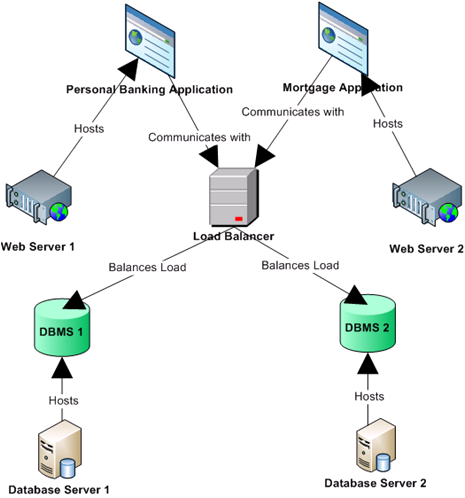
\includegraphics[width=7cm]{cmdbExample.PNG}
\caption{An IT System Stored in a CMDB}
\label{fig:cmdbExample}
\end{figure}

\subsection{Bayesian Networks}

\subsubsection{Tools}

\subsubsection*{Weka}

\subsubsection*{Banjo}
Banjo is a tool written in Java which infers the structure of a Bayesian network given training data. It has two different search algorithms: Greedy and
Simulated Annealing. For either of these search algorithms, it has two methods of proposing a new edge. The first is the ``proposeRandomLocalMove''
which basically proposes a random addition or removal of an edge. The other is ``proposeAllLocalMoves'' which proposes all possible moves, and only keeps the
best one (?). Banjo uses the BDe metric to compute a network's score.

\subsubsection*{JavaBayes}

\subsection{Evaluation Techniques}

We need a way to evaluate the predicted CIs. The recall and precision measures from the information retrieval field are appropriate for this type of evaluation.
Recall measures the proportion of correct CIs retrieved by the system, while precision measures the proportion of suggested CIs that are correct~\cite{van79}.

Similar to Hassan et. al~\cite{hassan2004predicting}, we define the \textit{Predicted Set} (P) as the set of all CIs DRACA suggests through the full the
iteration process (see Figure~\ref{fig:process}). We define the \textit{Occurred Set} (O) as the CIs remaining in the change set after excluding the Initial CI
provided by the analyst (i.e Change Set - Initial CI). The intersection of the predicted set and the occurred set, called $PO$, is the common CIs in both sets.
For each constructed change set, we then calculate the recall and precision values for the predictions according to the following
definitions~\cite{hassan2004predicting}:

\begin{equation}
\label{eqn:recall}
Recall = \frac{|PO|}{|O|}
\end{equation}

\begin{equation}
\label{eqn:precision}
Precision = \frac{|PO|}{|P|}
\end{equation}

If no CIs are predicted (i.e., $P$ and thus $PO$ are empty), precision is defined as 1 since there cannot exist any incorrect predictions in an empty set. On
the other hand, if the size of the change set is 1, and thus the size of the occurred set is 0, recall is defined as 1 since there are no CIs to
predict~\cite{hassan2004predicting}.  

In order to have a single measure that indicates the effectiveness of our predictions, we use the F-measure which is based on van Rijsbergen's effectiveness
measure which combines recall and precision~\cite{van79}. The F-measure is calculated according to Equation~\ref{eqn:f-measure} which gives equal weighting to
recall and precision. The ideal F-measure is 1 where both recall and precision are 1.

\begin{equation}
F = 2 * \frac{precision * recall}{precision +recall}
\label{eqn:f-measure}
\end{equation}

\section{Related Work}
\label{rel-work}

Mirarab et al.~\cite{mirarab2007} investigate the same problem as our work. However, their work is on the level of source code changes. They build three
different Bayesian Networks, one that is based on package and class dependency information (static relationships), one which is dependent on historical
co-changes, and one which uses both. For the first graph, the initial structure is essentially ``given'' according to the static dependencies, and then the CPTs
are learnt using the importance sampling algorithm proposed by Changhe and Marek~\cite{yuan2003importance}. The way static dependencies are defined in their
case is specific to Java. The third one is essentially the first graph, but updated using the historic change information according to the Expectation
Maximization (EM) algorithm~\cite{dempster1977maximum}. The second was solely based on historic information where the network is build using a greedy structure
 learning algorithm~\cite{friedman1996learning}. They did some preprocessing to their data such as filtering out large changes (with more than 30 elements
changed at once) since this was probably an insignificant change.

Zhou et al.~\cite{zhou2008} try to answer a slightly different problem. They do not only look at the probability of other elements changing given a specific
element, they also add features such as authors, change significance levels etc. and try to predict if two elements are co-changes or not accordingly. Thus,
their problem is more of a classification problem where given two elements, and some observed features they try to determine the class as co-changes or not.
They use the K2 algorithm proposed by Cooper et. al~\cite{cooper1992bayesian} to estimate the structure of the Bayesian network, and use the SimpleEstimator
algorithm built in WEKA~\cite{witten2005data}.

\section{Models Used}
\label{sec:modelsused}

In order to construct a Bayesian network which we can use to make predictions, there were two steps involved. First, determining the structure of the actual
network, and then estimating the Conditional Probability Tables (CPT). There were different ways in which we could estimate the structure of the network, and
so we built a model for each technique. However, for all models, we used the SimpleEstimator algorithm~\cite{written2005data} built in Weka to calculate the
CPTs. 

Before building any of the models, some data preprocessing was necessary. We first describe this preprocessing, and then proceed to explain each of the FOUR
models built.


\begin{figure}[!t]
\centering
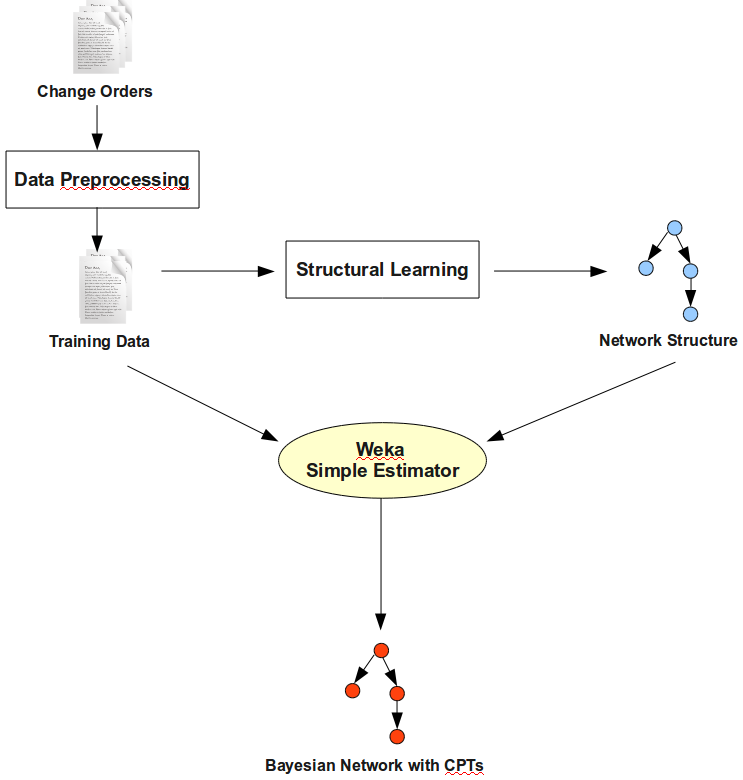
\includegraphics[width=7cm]{graphics/constructingmodel.png}
\caption{Generating the Bayesian Network}
\label{fig:process}
\end{figure}

\subsubsection{Data Preprocessing}
The original data set has 7,999 distinct CIs, and 27,305 change orders. This amount of data was infeasible to work with as no tool could handle such a large
amount of variables in a Bayesian network. For the purposes of this project, which is mainly to experiment with Bayesian techniques for change set prediction,
it is sufficient to choose a small representative subset of the data. Accordingly, in order to be able to test things properly, we used observations from three
months data from January 1, 2008 to March 31, 2008 to build the model. However, even in such a short period, there were already 2,841 distinct CIs appearing and
2,229 observations (i.e. change orders). Therefore, we needed to perform further data preprocessing. 

First, we removed all CIs that have changed less than 12 times within this time frame  (i.e were associated with 12 different change orders in our training
observations). There is no particular reason for choosing 12 as a cut off. It simply gave a feasible data set to deal with. This yielded 120 distinct CIs. Then,
in order to slightly increase our variable space to include other related CIs, we found all the parent CIs related to these 120 CIs from the CMDB perspective.
However, we ignored three common, and not extremely meaningful relations, which are  ``supports'', ``is location for'', and ``backs up''. Adding the related
parent CIs, we now had a set of 241 CIs. However, some of the added parent CIs may not be in the original set of 2,841 CIs. Accordingly, we just kept CIs tht
appeared more than 12 times or were in the set of related CIs. This provided us our final data set of 170 CIs which we use throughout our models for fair
comparison. Additionally, filtering out CIs meant filtering out some of the observations that did not have any CIs satisfying our criteria. This led to us
having 1,305 observations instead of 2,229 which was a more manegeable set. Accordingly, our training data set consisted of 170 variables (CIs), and 1,305
observations (change sets).

DESCRIBE GENERATED OBSERVATIONS FILE

FIGURE FOR DATA PROCESSING

\subsection{Model 1 (Banjo)}
\label{sec:model1}

For the first model, we used Banjo to learn the structure of the Bayesian network from the training data which used a Greedy searching algorithm. Banjo
produced five different top-scoring networks (having the same score), and we simply chose one of them as the network to be used. This network was then
formatted as an BIF XML file, and was fed into Weka's network analyzer tool. After setting the data set to be the observations in our training set, Weka
learned the CPTs for the network produced by Banjo. This complete network was then saved as an BIF XML file to be used by JavaBayes for general inference.


\subsection{Model 2 (CMDB Relationships)}

For the second model, we used the relations existing in the CMDB to infer the structure of the network (that is place the edges between the nodes). We used two
variations for this. The first was to follow the direction of the relationship edges in the CMDB. That is if there is an edge from A to B, we will place an
edge in the Bayesian network from A to B (we will call this model 2A). The second was to reverse the direction of the relationship edges in the CMDB. That is,
if there is an edge from A to B, we will place an edge in the Bayesian network from B to A (we will call this model 2B). In both cases, however, we chose to
ignore some relationship edges (WHY, TRY WITHOUT). There was one problem, however, with the generated network. Two of the CIs had more than 15 parents to them
which means that their CPTs will be intractable to compute. For those two CIs, we simply removed all their parents to make the computation tractable.


\subsection{Model 3 (Missing Data)}

This model is the same as the second model, except that we experimented with the missing data feature in Weka. Weka allows the user to specify missing values
for any variable by simply putting a '?' instead of its value. Therefore, instead of putting the CIs that did not appear in a change order as false, we put a
'?' in their place. This seemed closer to practice, because in reality, we are not sure whether this CI actually changed or not. Therefore, this model also has
two parts: model 3A and model 3B where the first uses the CMDB relationships in their same direction, and the second uses the reverse direction.

\begin{algorithm}[tb]
   \caption{Bubble Sort}
   \label{alg:example}
\begin{algorithmic}
   \STATE {\bfseries Input:} changeOrder
    \STATE {\bfseries Input:} BayesianNetwork
    \STATE {\bfseries Input:} threshold
    \STATE Set initialCI = first CI in changeOrder
    \STATE Set occurredSet = changeOrder - initialCI
    \STATE Initialize observedSet = {firstCI}
    \STATE Initialize predictedSet = {}
   \REPEAT  
    \STATE Initialize newPredictions = {}
    \FOR{$node$ {\bfseries to} $BayesianNetwork$}
    \STATE posterior = perform inference using Banjo
    \IF{$posterior > threshold$} 
      \STATE Add node to newPredictions   
    \ENDIF
    \ENDFOR

  \FOR{$prediction$ {\bfseries to} $newPredictions$}
    \IF{$prediction  occurredSet$}
      \STATE Add prediction to observedSet
    \ENDIF
    \ENDFOR
\STATE Add newPredictions to predictedSet

   \UNTIL{$newPredictions$ is $empty$}
\end{algorithmic}
\end{algorithm}


\section{Experimental Work}
\label{sec:exp}

\subsubsection*{Inference}

At this point, we have the Bayesian network ready, and we would like to perform Inference. More formally, given that a CI will change (our evidence), we want
to infer the probability that the other CIs in the network might change as well. Unfortunately, neither of the two tools previously used provide an Bayesian
inference engine. We, therefore, use JavaBayes in this step since it accepts the same ARFF format used by Weka. We using a one month testing set where we try
to predict all the change orders in April 2008 (883 reports). There was a total of XX change orders in that month. For each change order, we would take the
first CI as the initial CI to change, then we would set that as evidence, and update the beliefs of all the nodes (CIs) in the network using JavaBayes. We would
then loop on all the updated CIs, and add those that match our threshold criteria to the predicted change set. To simulate a real life scenario, we then checked
which of these predicted CIs actually lies in the target change set we are trying to predict. This is similar to an analyst accepting CIs into their change set.
These common CIs would then also be marked as observations so that we can predict now that I'm going to change B and C too, what else do I need to change.
Again, we would calculate the posterior probability, and continue doing so until there are no more common CIs. We would then calculate the recall, precision,
and F-measure accordingly.

\section{Conclusion}
\label{concl}


\bibliography{references}
\bibliographystyle{icml2010}

\end{document} 


